%% ro-crate paper
%% (c) 2020-2021 The University of Manchester
%% 
%% SPDX-License-Identifier: CC-BY-4.0


% add. options: [seceqn,secthm,crcready]
\documentclass[ds,crcready]{iosart2x}

%%%%%%%%%%% Put your definitions here

% From https://www.overleaf.com/latex/templates/using-the-stix2-opentype-fonts-with-lualatex-or-xelatex/hdfvhzqmhnpx
\usepackage{fontspec}
\usepackage{amsmath}
\usepackage{amssymb}
\usepackage{hyperref}
\usepackage{xcolor}
\definecolor{darkerblue}{cmyk}{1,1,0,0.45}
\hypersetup{
    colorlinks=true,
    linkcolor=black,
    citecolor=black,
    urlcolor=darkerblue}

\usepackage{unicode-math}
\usepackage{graphicx}

% Hyperlinks on DOI permalinks – just 20 years after DOI invention!
% 
% We had to make our own copy of 
% https://ctan.org/pkg/doi?lang=en 
% where commands are renamed to \doix
% because iosart2x.cls and ios1.bst have 
% a different use of \doiurl \doi etc.
% We also set the doixtext prefix empty
% to avoid doi:doi:
\usepackage{doix}
\renewcommand{\doixtext}{}
\renewcommand{\doiurl}[1]{\doix{#1}}

\DeclareGraphicsExtensions{.pdf,.png,.svg}
\graphicspath{../content/images/}
\usepackage[citations,definitionLists,fencedCode,footnotes,hybrid,pipeTables,smartEllipses,tableCaptions,underscores]{markdown}
\def\markdownOptionOutputDir{../output}
\def\markdownOptionHeaderAttributes{true}

% for table resizing
\usepackage{booktabs}
\usepackage{multirow}

%%%%%%%%%%% End of definitions


\pubyear{2022}
\volume{0}
\firstpage{1}
\lastpage{1}
\def\doi{10.3233/DS-210053}


\begin{document}

% Welcome to the 2000s with UNICODE fonts!
% Adapted from
% https://www.overleaf.com/learn/latex/Articles%2FOpenType-based_math_typesetting:_An_introduction_to_the_STIX2_OpenType_fonts
\setmathfont{STIX2Math}[
    Extension={.otf},
    Path=./STIX2fonts/,
    Scale=1
]
\setmainfont{STIX2Text}[
    Extension={.otf},
    Path=./STIX2fonts/,
    UprightFont={*-Regular},
    BoldFont={*-Bold},
    ItalicFont={*-Italic},
    BoldItalicFont={*-BoldItalic}
]

% https://typeof.net/Iosevka/ mono font has 
% all the logic symbols we need
%\setmonofont{iosevka-slab}[
%    Extension={.ttf},
%    Path=./ttf-iosevka-slab-6.1.3/,
%    Scale=MatchLowercase,
%    UprightFont={*-light},
%    ItalicFont={*-lightitalic}
%]

\begin{frontmatter}

%\pretitle{}
\title{Packaging research artefacts with RO-Crate}
\runtitle{Packaging research artefacts with RO-Crate}
%\subtitle{}

% For one author:
%\author{\inits{N.}\fnms{Name1} \snm{Surname1}\ead[label=e1]{first@somewhere.com}\ead[label=o1,orcid]{0000-0000-0000-0001}}
%\address{Department first, \orgname{University or Company name},
%Abbreviate US states, \cny{Country}\printead[presep={\\}]{e1,o1}}

% Two or more authors:
\author[SSR1,SSR2]{\inits{S.}\fnms{Stian}
    \snm{Soiland-Reyes}\ead[label=eSSR]{soiland-reyes@manchester.ac.uk}\ead[label=oSSR,orcid]{0000-0001-9842-9718}%
    \thanks{Corresponding author. \printead{eSSR}.}}, 
\author[PS]{\inits{P.}\fnms{Peter}
    \snm{Sefton}\ead[label=ePS]{Peter.Sefton@uts.edu.au}\ead[label=oPS,orcid]{0000-0002-3545-944X}},
\author[MC]{\inits{M.}\fnms{Mercè}
    \snm{Crosas}\ead[label=eMC]{mcrosas@g.harvard.edu}\ead[label=oMC,orcid]{0000-0003-1304-1939}},
\author[LJC]{\inits{LJ.}\fnms{Leyla Jael}
    \snm{Castro}\ead[label=eLJC]{ljgarcia@zbmed.de}\ead[label=oLJC,orcid]{0000-0003-3986-0510}},
\author[FC]{\inits{F.}\fnms{Frederik}
    \snm{Coppens}\ead[label=eFC]{frcop@psb.vib-ugent.be}\ead[label=oFC,orcid]{0000-0001-6565-5145}},
\author[JMF]{\inits{JM.}\fnms{José M.}
    \snm{Fernández}\ead[label=eJMF]{jose.m.fernandez@bsc.es}\ead[label=oJMF,orcid]{0000-0002-4806-5140}},
\author[DG]{\inits{D.}\fnms{Daniel}
    \snm{Garijo}\ead[label=eDG]{dgarijo@fi.upm.es}\ead[label=oDG,orcid]{0000-0003-0454-7145}},
\author[BG]{\inits{B.}\fnms{Björn}
    \snm{Grüning}\ead[label=eBG]{gruening@informatik.uni-freiburg.de}\ead[label=oBG,orcid]{0000-0002-3079-6586}},
\author[MLR]{\inits{M.}\fnms{Marco}
    \snm{La Rosa}\ead[label=eMLR]{m@lr.id.au}\ead[label=oMLR,orcid]{0000-0001-5383-6993}},
\author[SL]{\inits{S.}\fnms{Simone}
    \snm{Leo}\ead[label=eSL]{simone.leo@crs4.it}\ead[label=oSL,orcid]{0000-0001-8271-5429}},
\author[EOC]{\inits{E.}\fnms{Eoghan}
    \snm{Ó Carragáin}\ead[label=eEOC]{eoghan.ocarragain@ucc.ie}\ead[label=oEOC,orcid]{0000-0001-8131-2150}},
\author[MP]{\inits{M.}\fnms{Marc}
    \snm{Portier}\ead[label=eMP]{marc.portier@vliz.be}\ead[label=oMP,orcid]{0000-0002-9648-6484}},
\author[AT]{\inits{A.}\fnms{Ana}
    \snm{Trisovic}\ead[label=eMP]{ana.trisovic@gmail.com}\ead[label=oAT,orcid]{0000-0003-1991-0533}},
\author[RO]{RO-Crate Community},
\author[PG]{\inits{P.}\fnms{Paul}
    \snm{Groth}\ead[label=ePG]{p.t.groth@uva.nl}\ead[label=oPG,orcid]{0000-0003-0183-6910}},
\author[CG]{\inits{C.}\fnms{Carole}
    \snm{Goble}\ead[label=eCG]{carole.goble@manchester.ac.uk}\ead[label=oCG,orcid]{0000-0003-1219-2137}}

\address[SSR1]{Department of Computer Science, 
    \orgname{The University of Manchester}, \cny{UK}\printead[presep={\\}]{eSSR,oSSR}}
\address[SSR2]{Informatics Institute, \orgname{University of Amsterdam},
    \cny{The Netherlands}}
\address[PS]{Faculty of Science, \orgname{University Technology Sydney},
    \cny{Australia}\printead[presep={\\}]{ePS,oPS}}
\address[MC]{Institute for Quantitative Social Science, 
    \orgname{Harvard University}, Cambridge, MA,  \cny{USA}\printead[presep={\\}]{oMC}}
\address[LJC]{\orgname{ZB MED Information Centre for Life Sciences}, 
    Cologne, \cny{Germany}\printead[presep={\\}]{oLJC}}
\address[FC]{\orgname{VIB-UGent Center for Plant Systems Biology}, 
    Gent, \cny{Belgium}\printead[presep={\\}]{oFC}}
\address[JMF]{\orgname{Barcelona Supercomputing Center}, 
    Barcelona, \cny{Spain}\printead[presep={\\}]{oJMF}}
\address[DG]{Ontology Engineering Group, 
    \orgname{Universidad Politécnica de Madrid}, Madrid, \cny{Spain}\printead[presep={\\}]{oDG}}
\address[BG]{Bioinformatics Group, Department of Computer Science,
    \orgname{Albert-Ludwigs-University Freiburg}, Freiburg, \cny{Germany}\printead[presep={\\}]{oBG}}
\address[MLR]{\orgname{PARADISEC}, Melbourne, \cny{Australia}\printead[presep={\\}]{oMLR}}
\address[SL]{\orgname{Center for Advanced Studies, Research, and Development in Sardinia} (CRS4), Pula (CA),
    \cny{Italy}\printead[presep={\\}]{oSL}}
\address[EOC]{\orgname{University College Cork},
    \cny{Ireland}\printead[presep={\\}]{oEOC}}
\address[MP]{\orgname{Vlaams Instituut voor de Zee}, Oostende,
    \cny{Belgium}\printead[presep={\\}]{oMP}}
\address[AT]{Institute for Quantitative Social Science,
    \orgname{Harvard University}, Cambridge, MA, \cny{USA}\printead[presep={\\}]{oAT}}
\address[RO]{\url{https://www.researchobject.org/ro-crate/community} (see appendix B)}
\address[PG]{Informatics Institute, \orgname{University of Amsterdam},
    \cny{The Netherlands}\printead[presep={\\}]{ePG,oPG}}
\address[CG]{Department of Computer Science, \orgname{The University of Manchester},
    \cny{UK}\printead[presep={\\}]{eCG,oCG}}
    
%\begin{review}{editor}
%\reviewer{\fnms{First} \snm{Editor}\ead[label=oe1,orcid]{}\printead[presep={\ }]{oe1}}
%\reviewer{\fnms{Second} \snm{Editor}\ead[label=oe2,orcid]{}\printead[presep={\ }]{oe2}}
%\end{review}
%\begin{review}{solicited}
%\reviewer{\fnms{First} \snm{Solicited reviewer}\ead[label=os1,orcid]{}\printead[presep={\ }]{os1}}
%\end{review}

\begin{abstract}
\markdownInput{../content/01.abstract.md}
\end{abstract}

\begin{keyword}
\kwd{Data publishing}
\kwd{Data packaging}
\kwd{FAIR}
\kwd{Linked Data}
\kwd{Metadata}
\kwd{Reproducibility}
\kwd{Research Object}
\end{keyword}

\end{frontmatter}

%%%%%%%%%%% The article body starts:

% Every *.md file in content/ in order, except 00, 90
\markdownInput{../content/10.background.md}

\markdownInput{../content/20.rocrate.md}
%% sub-subsections below to cater for figures in 
%% markdown vs LaTex
\markdownInput{../content/20a.methodology.md}
\markdownInput{../content/21.conceptual.md}
\begin{figure}[t!]
    \centering
    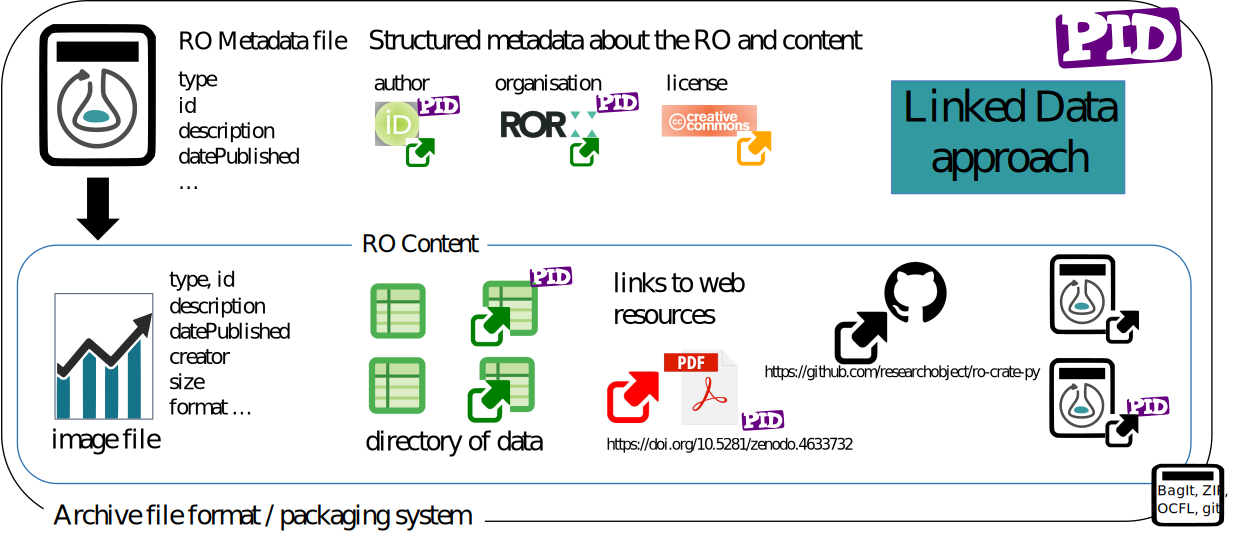
\includegraphics[width=0.95\textwidth]{content/images/ro-crate-overview.pdf}
\caption{\textbf{Conceptual overview of RO-Crate}. A \emph{Persistent Identifier} (PID) \cite{doi:10.1371/journal.pbio.2001414} points to a \emph{Research Object} (RO), which may be archived using different packaging approaches like BagIt \cite{doi:10.17487/rfc8493}, OCFL \cite{ocfl_2020}, git or ZIP. The RO is described within a \emph{RO-Crate Metadata File}, providing identifiers for \emph{authors} using ORCID, \emph{organisations} using ROR \cite{doi:10.6087/kcse.192} and licences such as Creative Commons using SPDX identifiers. The \emph{RO-Crate content} is further described with additional metadata following a Linked Data approach. Data can be embedded files and directories, as well as links to external web resources, PIDs and nested RO-Crates.}
    \label{fig:conceptual}
\end{figure}

\markdownInput{../content/21b.foundation.md}
\markdownInput{../content/21c.container.md}
\markdownInput{../content/21d.contextual-entities.md}

\begin{figure}[t!]
    \centering
    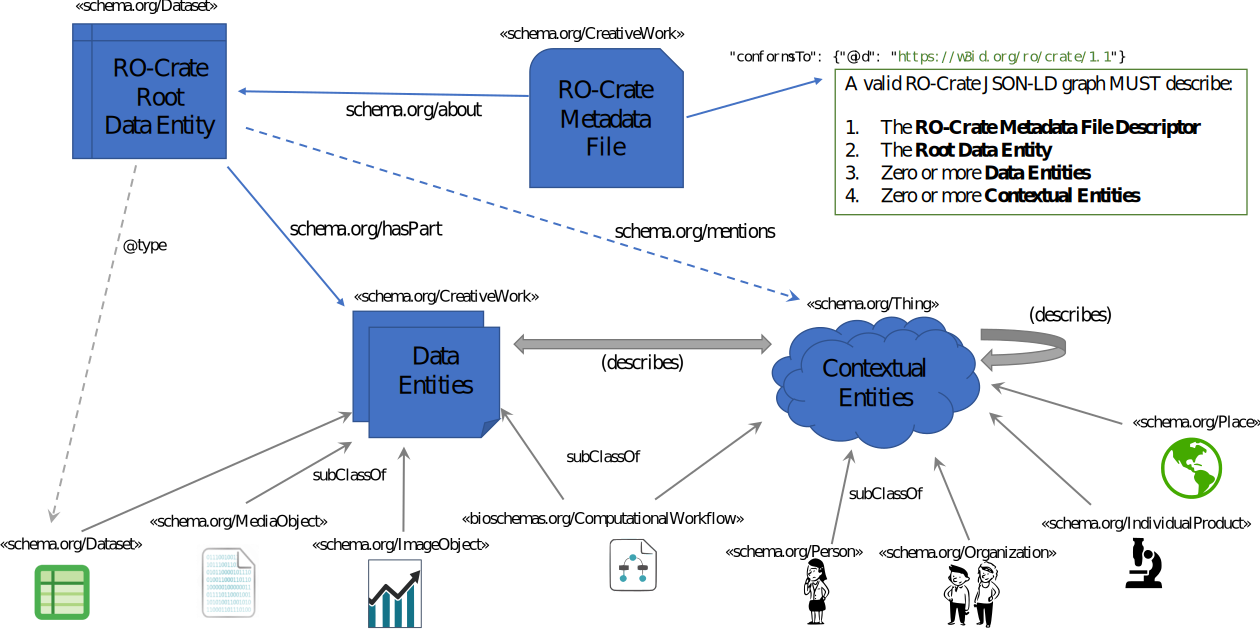
\includegraphics[width=0.9\textwidth]{content/images/ro-crate-uml.pdf}
    \caption{\textbf{Simplified UML class diagram of RO-Crate.} The \emph{RO-Crate Metadata File} conforms to a version of the specification; and contains a JSON-LD graph \cite{sporny_2014} that describes the entities that make up the RO-Crate. The \emph{RO-Crate Root Data Entity} represent the Research Object as a dataset. The RO-Crate aggregates \emph{data entities} (\texttt{hasPart}) which are further described using \emph{contextual entities} (which may include aggregated and non-aggregated data entities). Multiple types and relations from Schema.org allow annotations to be more specific, including figures, nested datasets, computational workflows, people, organisations, instruments and places. Contextual entities not otherwise cross-referenced from other entities' properties (\emph{describes}) can be grouped under the root entity (\texttt{mentions}).}
    \label{fig:uml}
\end{figure}

\markdownInput{../content/21f.guiding-practices.md}
\markdownInput{../content/21g.simplicity.md}
\markdownInput{../content/21h.extensibility.md}

\markdownInput{../content/22.implementation.md}
\markdownInput{../content/23.community.md}

% Please update in 31.tooling-table.md first!
\begin{table}[htbp]
	\centering
	\begin{tabular}{llll}
		\toprule
		\textbf{Tool name} & Targets & Language / Platform & Status \\
		\multicolumn{4}{l}{\it Brief Description} \\
		\midrule
		
		\textbf{Describo} \citep{describo} & Research Data Managers & NodeJS (Desktop) & RC \\
		\multicolumn{4}{l}{\it Interactive desktop application to create, update and export RO-Crates for different profiles} \\
		
		\textbf{Describo Online} \citep{describo-online} & Platform developers & NodeJS (Web) & Alpha \\
		\multicolumn{4}{l}{\it Web-based application to create RO-Crates using cloud storage} \\
		
		\textbf{ro-crate-excel} \citep{ro-crate-excel} & Data managers & JavaScript \\
		\multicolumn{4}{l}{\it Command-line tool to help create RO-Crates and HTML-readable rendering} \\
		
		\textbf{ro-crate-html-js} \citep{ro-crate-html-js} & Developers & JavaScript & Beta \\
		\multicolumn{4}{l}{\it HTML rendering of RO-Crate}  \\
		
		\textbf{ro-crate-js} \citep{ro-crate-js} & Research Data Managers & JavaScript & Alpha \\
		\multicolumn{4}{l}{\it Library for creating/manipulating crates; basic validation code} \\
		
		\textbf{ro-crate-ruby} \citep{ro-crate-ruby} & Developers & Ruby & Beta \\
		\multicolumn{4}{l}{\it Ruby library for reading/writing RO-Crate, with workflow support} \\
		
		\textbf{ro-crate-py} \citep{ro-crate-py} & Developers & Python & Beta \\
		\multicolumn{4}{l}{\it Object-oriented Python library for reading/writing RO-Crate} \\
		
		\textbf{WorkflowHub} \citep{about-workflowhub} & Workflow users & Ruby & Beta \\
		\multicolumn{4}{l}{\it Workflow repository; imports and exports Workflow RO-Crate} \\
		
		\textbf{Life Monitor} \citep{about-lifemonitor} & Workflow developers & Python & Alpha \\
		\multicolumn{4}{l}{\it Workflow testing and monitoring service; Workflow Testing profile of RO-Crate} \\
		
        \textbf{SCHeMa} \citep{arxiv:2103.13138v1} & Workflow users & PHP & Alpha \\
        \multicolumn{4}{l}{\it Workflow execution using RO-Crate as exchange mechanism} \\

		\textbf{galaxy2cwl} \citep{galaxy2cwl} & Workflow developers & Python & Alpha \\
		\multicolumn{4}{l}{\it Wraps Galaxy workflow as Workflow RO-Crate} \\

		\textbf{Modern PARADISEC} \citep{modpdsc} & Repository managers & Platform & Beta \\
		\multicolumn{4}{l}{\it Cultural Heritage portal based on OCFL and RO-Crate} \\
		
		\textbf{ONI express} \citep{arkisto-data-portal} & Repository managers & Platform & Beta \\
		\multicolumn{4}{l}{\it Platform for publishing data and documents stored in an OCFL repository via a web interface} \\
		
		\textbf{ocfl-tools} \citep{ocfl-tools} & Developers & JavaScript (CLI) & Beta \\
		\multicolumn{4}{l}{\it Tools for managing RO-Crates in an OCFL repository}\\
		
		\textbf{RO Composer} \citep{ro-composer} & Repository developers & Java & Alpha \\ 
		\multicolumn{4}{l}{\it REST API for gradually building ROs for given profile} \\
		
		\textbf{RDA maDMP Mapper} \citep{doi:10.5281/zenodo.3922136} & Data Management Plan users & Python & Beta \\
		\multicolumn{4}{l}{\it Mapping between machine-actionable data management plans (maDMP) and RO-Crate\citep{doi:10.4126/frl01-006423291} } \\

        \textbf{Ro-Crate\_2\_ma-DMP} \citep{doi:10.5281/zenodo.3903463} & Data Management Plan users & Python & Beta \\
        \multicolumn{4}{l}{\it Convert between machine-actionable data management plans (maDMP) and RO-Crate } \\
        
        \textbf{CheckMyCrate} \citep{CheckMyCrate} & Developers & Python (CLI) & Alpha \\
        \multicolumn{4}{l}{\it Validation according to Workflow RO-Crate profile} \\

		\bottomrule
	\end{tabular}
	\caption{Applications and libraries implementing RO-Crate, targeting different types of users across multiple programming languages. Status is indicative as assessed by this work (Alpha < Beta < Release Candidate (RC) < Release).}
	\label{tab:tools}
\end{table}
\markdownInput{../content/30.tooling.md}

\markdownInput{../content/40.inuse.md}
\markdownInput{../content/41.workflows.md}
\markdownInput{../content/42.regulatory.md}
\begin{figure}[t]
    \centering
    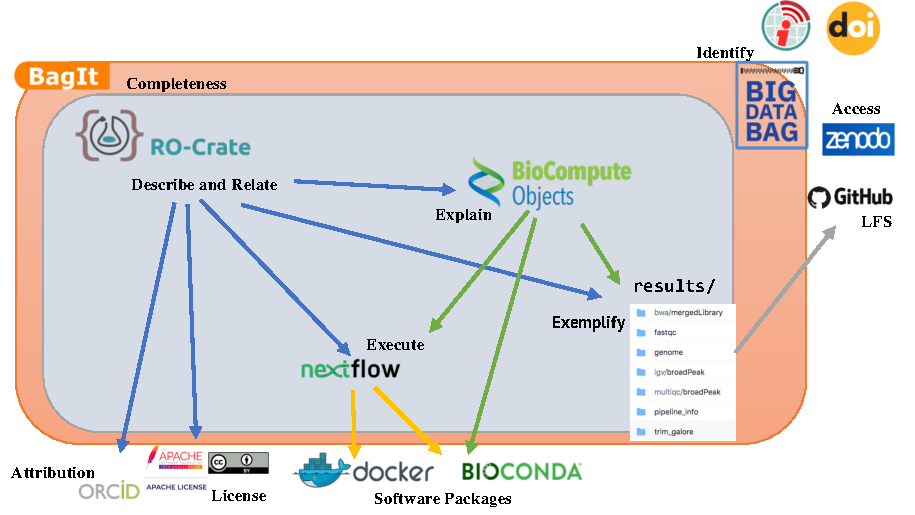
\includegraphics{content/images/ro-crate-bco-sep-of-concerns.pdf}
    \caption{\textbf{Separation of Concerns in BCO RO-Crate}. BioCompute Object (IEEE2791) is a JSON file that structurally explains the purpose and implementation of a computational workflow, for instance implemented in Nextflow, that installs the workflow’s software dependencies as Docker containers or BioConda packages. An example execution of the workflow shows the different kinds of result outputs, which may be external, using GitHub LFS to support larger data. RO-Crate gathers all these local and external resources, relating them and giving individual descriptions, for instance permanent DOI identifiers for reused datasets accessed from Zenodo, but also adding external identifiers to attribute authors using ORCID or to identify which licences apply to individual resources. The RO-Crate and its local files are captured in a BagIt whose checksum ensures completeness, combined with Big Data Bag \cite{doi:10.1109/BigData.2016.7840618} features to “complete” the bag with large external files such as the workflow outputs}
    \label{fig:sep_concerns}
\end{figure}
\markdownInput{../content/43.culturalheritage.md}
\markdownInput{../content/44.dmp.md}
\markdownInput{../content/45.institutional-repos.md}

\begin{figure}[t!]
    \centering
    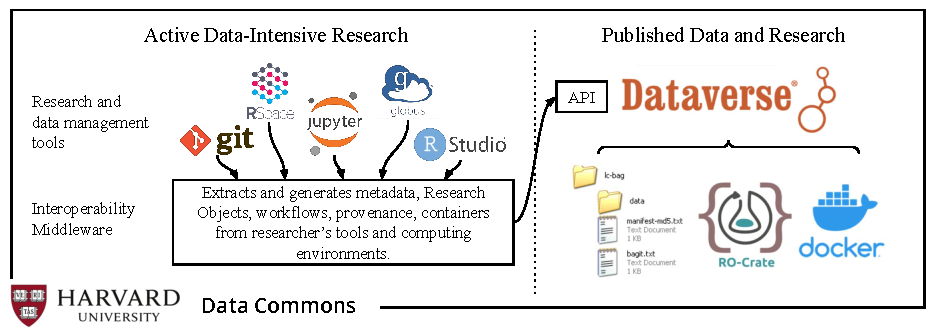
\includegraphics{content/images/data-commons-ro-crate-figure-5.pdf}
    \caption{\textbf{One aspect of Harvard Data Commons}. Automatic encapsulation and deposit of artefacts from data management tools used during active research at the Harvard Dataverse repository.}
    \label{fig:hdc}
\end{figure}


\markdownInput{../content/50.relatedwork.md}

\markdownInput{../content/60.conclusion.md}
\markdownInput{../content/61.futurework.md}

\markdownInput{../content/70.acknowledgements.md}




%%%% Appendix

\newpage
\appendix
%\markdownInput{../content/80.formal-definition.md}
% Because this file is added with \include, do not use
% Markdown setions within.
%
% Edit here before syncing to 80.formal-definition.md for HTML version


\section{Formalizing RO-Crate in First Order Logic}

\label{sec:formaldefinition}

Below is a formalization of the concept of RO-Crate as a set of relations using First Order Logic:

\subsection{Language}

Definition of language $\mathcal{L}_{rocrate}$:

\begin{eqnarray*}
    \mathcal{L}_{rocrate}   & = & \big\{ Property(p), Class(c),
                            Value(x), \mathbb{R}, \mathbb{S} \big\} \\
    \mathbb{D}              & = & \mathbb{IRI} \\
    \mathbb{IRI}            & \equiv & { \text{IRIs as defined in RFC3987} } \\
    \mathbb{R}              & \equiv & { \text{real or integer numbers} } \\
    \mathbb{S}              & \equiv & { \text{literal strings} }
\end{eqnarray*}


The domain of discourse $\mathbb{D}$ is the set of $\mathbb{IRI}$ identifiers \cite{doi:10.17487/rfc3987} (notation $\texttt{<http://example.com/>}$)\footnote{
    For simplicity, blank nodes are not included in this formalisation, as RO-Crate
    recommends the use of IRI identifiers: \url{https://www.researchobject.org/ro-crate/1.1/appendix/jsonld.html\#describing-entities-in-json-ld}
}, with additional descriptions using numbers $\mathbb{R}$ (notation $13.37$) and literal strings $\mathbb{S}$ (notation $\text{“Hello”}$).

From this formalised language $\mathcal{L}_{rocrate}$ we can interpret an RO-Crate in any representation that can gather these descriptions, their properties, classes, and literal attributes.

\subsection{Minimal RO-Crate}

Below we use $\mathcal{L}_{rocrate}$ to define a minimal\footnote{
    The full list of types, relations and attribute properties from the RO-Crate specification are not included. Examples shown include $datePublished$, $CreativeWork$ and $name$.
} RO-Crate:


\begin{eqnarray*}
ROCrate(R)                                  & \models & Root(R) \land Mentions(R, R) \land hasPart(R, d) \land \\
                                            & & Mentions(R, d) \land DataEntity(d) \land \\
                                            & & Mentions(R, c) \land ContextualEntity(c) \\
\forall r \ Root(r)                         & \Rightarrow & Dataset(r) \land name(r, n) \land description(r, d) \land \\
                                            & &             datePublished(r, date) \land license(e, l) \\
\forall e \forall n \ name(e, n)            & \Rightarrow & Value(n) \\
\forall e \forall s \ description(e, s)     & \Rightarrow & Value(s) \\
\forall e \forall d \ datePublished(e, d)   & \Rightarrow & Value(d) \\
\forall e \forall l \ license(e, l)         & \Rightarrow & ContextualEntity(l) \\
DataEntity(e)                               & \equiv &      File(e) \oplus Dataset(e) \\
Entity(e)                                   & \equiv &      DataEntity(e) \lor ContextualEntity(e) \\
\forall e \ Entity(e)                       & \Rightarrow & type(e, c) \land Class(c) \\
\forall e \ ContextualEntity(e)             & \Rightarrow & name(e, n)  \\
Mentions(R, s)                              & \models &     Relation(s, p, e) \oplus Attribute(s,  p, l) \\
Relation(s, p, o)                           & \models &     Entity(s) \land Property(p) \land  Entity(o) \\
Attribute(s, p, v)                          & \models &     Entity(s) \land Property(p) \land Value(v) \\
Value(v)                                    & \equiv &      v \in \mathbb{R} \oplus v \in \mathbb{S}
\end{eqnarray*}

An $ROCrate(R)$ is defined as a self-described \emph{Root Data Entity}, which describes and contains parts (\emph{data entities}), which are further described in \emph{contextual entities}.  These terms align with their use in the RO-Crate 1.1 terminology\footnote{
    \url{https://www.researchobject.org/ro-crate/1.1/terminology}}.

The $Root(r)$ is a type of $Dataset(r)$, and must have the metadata to literal attributes to provide a $name$, $description$ and $datePublished$, as well as a contextual entity identifying its license. These predicates correspond to the RO-Crate 1.1 requirements for the root data entity\footnote{
    \url{https://www.researchobject.org/ro-crate/1.1/root-data-entity.html\#direct-properties-of-the-root-data-entity}
}.

The concept of an $Entity(e)$ is introduced as being either a $DataEntity(e)$, a $ContextualEntity(e)$, or both\footnote{
    \url{https://www.researchobject.org/ro-crate/1.1/contextual-entities.html\#contextual-vs-data-entities}
}. Any $Entity(e)$ must be typed with at least one $Class(c)$, and every $ContextualEntity(e)$ must also have a $name(e,n)$; this corresponds to expectations for any \emph{referenced contextual entity} (section \ref{sec:contextualentities}). 

For simplicity in this formalization (and to assist production rules below) $R$ is a constant representing a single RO-Crate, typically written to independent RO-Crate Metadata files. $R$ is used by $Mentions(R, e)$ to indicate that $e$ is an Entity described by the RO-Crate and therefore its metadata (a set of $Relation$ and $Attribute$ predicates) form part of the RO-Crate serialization. $Relation(s, p, o)$ and $Attribute(s, p, x)$ are defined as a \emph{subject—predicate—object} triple pattern from an $Entity(s)$ using a $Property(p)$ to either another $Entity(o)$ or a $Value(x)$ value.

\subsection{Example of formalized RO-Crate}

The below is an example RO-Crate represented using the above formalisation, assuming a base URI of \texttt{<http://example.com/ro/123/>}:

\allowdisplaybreaks
\begin{eqnarray*}
&& ROCrate(\texttt{<http://example.com/ro/123/>}) \\
&& name(\texttt{<http://example.com/ro/123/>}, \\
&& \ \ \ \ \ \text{“Data files associated with the manuscript:Effects of …”}) \\
&& description(\texttt{<http://example.com/ro/123/}, \\
&& \ \ \ \ \ \text{“Palliative care planning for nursing home residents …”}) \\
&& license(\texttt{<http://example.com/ro/123/>}, \\
&& \ \ \ \ \ \texttt{<https://spdx.org/licenses/CC-BY-4.0>}) \\
&& datePublished(\texttt{<http://example.com/ro/123/>}, \text{“2017-02-23”}) \\
&& hasPart(\texttt{<http://example.com/ro/123/>},
        \texttt{<http://example.com/ro/123/file.txt>}) \\
&& hasPart(\texttt{<http://example.com/ro/123/>},
        \texttt{<http://example.com/ro/123/interviews/>}) \\
\\
&& ContextualEntity(\texttt{<https://spdx.org/licenses/CC-BY-4.0>}) \\
&& name(\texttt{<https://spdx.org/licenses/CC-BY-4.0>},  \\
&& \ \ \ \ \  \text{Creative Commons Attribution 4.0”}) \\
\\
&& ContextualEntity(\texttt{<https://spdx.org/licenses/CC-BY-NC-4.0>}) \\
&& name(\texttt{<https://spdx.org/licenses/CC-BY-NC-4.0>},  \\
&& \ \ \ \ \  \text{Creative Commons Attribution Non Commercial 4.0”}) \\
\\
&& File(\texttt{<http://example.com/ro/123/survey.csv>}) \\
&& name(\texttt{<http://example.com/ro/123/survey.csv>},
        \text{“Survey of care providers”}) \\
\\
&& Dataset(\texttt{<http://example.com/ro/123/interviews/>}) \\
&& name(\texttt{<http://example.com/ro/123/interviews/>},  \\
&& \ \ \ \ \  \text{“Audio recordings of care provider interviews”}) \\
&& license(\texttt{<http://example.com/ro/123/interviews/>}, \\
&& \ \ \ \ \ \texttt{<https://spdx.org/licenses/CC-BY-NC-4.0>})
\end{eqnarray*}


Notable from this triple-like formalization is that a RO-Crate $R$ is fully represented as a tree at depth 2 helped by the use of $𝕀𝕣𝕚$ nodes. For instance the aggregation from the root entity $hasPart(\texttt{…interviews/>})$ is at same level as the data entity’s property $license(\texttt{…CC-BY-NC-4.0>})$ and that contextual entity’s attribute $ name(\text{…Non Commercial 4.0”})$. As shown in section \ref{sec:jsonld}, the RO-Crate Metadata File serialization is an equivalent shallow tree, although at depth 3 to cater for the JSON-LD preamble of \texttt{"@context"} and \texttt{"@graph"}.

In reality many additional attributes and contextual types from Schema.org types like \url{http://schema.org/affiliation} and \url{http://schema.org/Organization} would be used to further describe the RO-Crate and its entities, but as these are optional (\textit{SHOULD} requirements) they do not form part of this formalization.


\subsection{Mapping to RDF with Schema.org}

A formalized RO-Crate in $\mathcal{L}_{rocrate}$ can be mapped to different serializations.
Assume a simplified\footnote{
 This simplification does not cover the extensive list of literal datatypes built-in to RDF 1.1, only strings and decimal real numbers. Likewise, language of literals are not included.
} language $\mathcal{L}_{RDF}$
based on the RDF abstract syntax \cite{rdfworkinggroup_2014}:

\begin{eqnarray*}
\mathcal{L}_{RDF}           & \equiv &      \big\{ Triple(s,p,o), IRI(i), BlankNode(b), Literal(s),
    \mathbb{IRI}, \mathbb{S}, \mathbb{R}    \big\} \\
\mathbb{D}_{RDF}            & \equiv &      \mathbb{S} \\
\forall i \ IRI(i)          & \Rightarrow & i \in \mathbb{IRI} \\
\forall s \forall p \forall o \
    Triple(s,p,o)           & \Rightarrow & \Big( IRI(s) \lor BlankNode(s) \Big) \land  \\
                            & &             IRI(p) \land  \\
                            & &             \Big(IRI(o) \lor BlankNode(o) \lor Literal(o) \Big) \\
Literal(v)                  & \models &     Value(v) \land Datatype(v,t) \land IRI(t) \\
\forall v \ Value(v)        & \Rightarrow & v \in \mathbb{S} \\
LanguageTag(v, l)           & \equiv &      Datatype\big(v, \\
    && \texttt{<http://www.w3.org/1999/02/22-rdf-syntax-ns\#langString>}\big)
\end{eqnarray*}

Below follows a mapping from $\mathcal{L}_{rocrate}$ to $\mathcal{L}_{RDF}$ using Schema.org as vocabulary:

\begin{eqnarray*}
Property(p)         & \Rightarrow &     type(p, \texttt{<http://www.w3.org/2000/01/rdf-schema\#Property>})   \\
Class(c)            & \Rightarrow &     type(c, \texttt{<http://www.w3.org/2000/01/rdf-schema\#Class>})  \\
Dataset(d)          & \Rightarrow &     type(d, \texttt{<http://schema.org/Dataset>})   \\
File(f)             & \Rightarrow &     type(f, \texttt{<http://schema.org/MediaObject>})   \\
ContextualEntity(e) & \Rightarrow &     type(f, \texttt{<http://schema.org/Thing>})   \\
CreativeWork(e)     & \Rightarrow &     ContextualEntity(e) \land type(e, \texttt{<http://schema.org/CreativeWork>})  \\
hasPart(e, t)       & \Rightarrow &     Relation(e, \texttt{<http://schema.org/hasPart>}, t)    \\
name(e, n)          & \Rightarrow &     Attribute(e, \texttt{<http://schema.org/name>}, n)  \\
description(e, s)   & \Rightarrow &     Attribute(e, \texttt{<http://schema.org/description>}, s)   \\
datePublished(e, d) & \Rightarrow &     Attribute(e, \texttt{<http://schema.org/datePublished>}, d) \\
license(e, l)       & \Rightarrow &     Relation(e, \texttt{<http://schema.org/license>}, l) \land CreativeWork(l) \\
type(e, t)          & \Rightarrow &     Relation(e, \texttt{<http://www.w3.org/1999/02/22-rdf-syntax-ns\#type>}, t) \\
                    & & \land Class(t)   \\
String(s)           & \equiv &          Value(s) \land  s \in \mathbb{S} \\
String(s)           & \Rightarrow &     Datatype(s, \texttt{<http://www.w3.org/2001/XMLSchema\#string>}) \\
Decimal(d)          & \equiv &          Value(d) \land  d \in \mathbb{R} \\
Decimal(d)          & \Rightarrow &     Datatype(d, \texttt{<http://www.w3.org/2001/XMLSchema\#decimal>}) \\
Relation(s,p,o)     & \Rightarrow &     Triple(s,p,o) \land IRI(s) \land IRI(o) \\
Attribute(s,p,o)    & \Rightarrow &     Triple(s,p,o) \land IRI(s) \land Literal(o) \\
\end{eqnarray*}

Note that in the JSON-LD serialization of RO-Crate, the expression of $Class$ and $Property$ is typically indirect: The JSON-LD \texttt{@context} maps to Schema.org IRIs, which, when resolved as Linked Data, embed their formal definition as RDFa. Extensions may however include such term definitions directly in the RO-Crate.

\subsection{RO-Crate 1.1 Metadata File Descriptor}

An important RO-Crate principle is that of being \textbf{self-described} Therefore the serialisation of the RO-Crate into a file should also describe itself in a Metadata File Descriptor\footnote{
    \url{https://www.researchobject.org/ro-crate/1.1/root-data-entity.html\#ro-crate-metadata-file-descriptor}
}, indicating it is $about$ (describing) the RO-Crate root data entity, and that it $conformsTo$ a particular version of the RO-Crate specification:

\begin{eqnarray*}
about(s,o)      & \Rightarrow & Relation(s, \texttt{<http://schema.org/about>}, o)   \\
conformsTo(s,o) & \Rightarrow & Relation(s, \texttt{<http://purl.org/dc/terms/conformsTo>}, o)   \\
MetadataFile(m) & \Rightarrow & CreativeWork(m) \land about(m,R) ∧ ROCrate(R) \land    \\
                &             & conformsTo(m, \texttt{<https://w3id.org/ro/crate/1.1>})
\end{eqnarray*}

Note that although the metadata file necessarily is an \emph{information resource} written to disk or served over the network (as JSON-LD), it is not considered to be a contained \emph{part} of the RO-Crate in the form of a \emph{data entity}, rather it is described only as a \emph{contextual entity}.

In the conceptual model the \emph{RO-Crate Metadata File} can be seen as the top-level node that describes the \emph{RO-Crate Root}, however in the formal model (and the JSON-LD format) the metadata file descriptor is an additional contextual entity that is not affecting the depth-limit of the RO-Crate.

\subsection{Forward-chained Production Rules for JSON-LD}

Combining the above predicates and Schema.org mapping with rudimentary JSON templates, these forward-chaining production rules can output JSON-LD according to the RO-Crate 1.1 specification\footnote{
    \textbf{Limitations:} Contextual entities not related from the RO-Crate (e.g. using inverse relations to a data entity) would not be covered by the single direction $Mentions(R, s)$ production rule; see \href{https://github.com/ResearchObject/ro-crate/issues/122}{GitHub issue ResearchObject/ro-crate\#122}. The $datePublished(e, d)$ rule do not include syntax checks for the ISO 8601 datetime format. Compared with RO-Crate examples, this generated JSON-LD does not use a $@context$ as the IRIs are produced unshortened, a post-step could do JSON-LD Flattening with a versioned RO-Crate context. The \texttt{@type} expansion is included for clarity, even though this is also implied by the $type(e, t)$ expansion to $Relation(e, \texttt{xsd:type})$.
}:

\begin{eqnarray*}
Mentions(R, s) \land Relation(s,p,o)
                        & \Rightarrow & Mentions(R, o) \\
IRI(i)                  & \Rightarrow & \texttt{"} i \texttt{"} \\
Decimal(d)              & \Rightarrow & d \\
String(s)               & \Rightarrow & \texttt{"} s \texttt{"} \\
\forall e \forall t
\ type(e, t)            & \Rightarrow & \texttt{\{"@id":}  e \texttt{,} \\
&&                               \ \  \texttt{"@type":} t \\
&&                              \texttt{\}} \\
\forall s \forall p \forall o
\ Relation(s,p,o)
                        & \Rightarrow &  \texttt{\{"@id":}  s \texttt{,} \\
&&                               \ \  p \texttt{: \{ "@id":} o \texttt{\}} \\
&&                              \texttt{\}} \\
\forall s \forall p \forall v
\ Attribute(s,p,v)    & \Rightarrow &  \texttt{\{"@id":} s \texttt{,} \\
&&                               \ \ p \texttt{:} v  \\
&&                               \texttt{\}} \\
\forall r  \forall c
    ROCrate(r)      & \Rightarrow &  \texttt{\{ "@graph": [} \\
&& \ \ \ \ Mentions(r, c)* \\
&& \ \ \ \texttt{]} \\
&& \texttt{\}} \\
R   & \equiv & \texttt{<./>}  \\
R   & \Rightarrow &  MetadataFile(\texttt{<ro-crate-metadata.json>}) \\
\end{eqnarray*}

This exposes the first order logic domain of discourse of IRIs, with rational numbers and strings as their corresponding JSON-LD representation. These production rules first grow the graph of $R$ by adding a transitive rule – anything described in $R$ which is related to $o$, means that $o$ is also mentioned by the $ROCrate(R)$. For simplicity this rule is one-way; in theory the graph can also contain free-standing contextual entities that have outgoing relations to data- and contextual entities, but these are proposed to be bound to the root data entity with Schema.org relation \href{http://schema.org/mentions}.


\newpage
\markdownInput{../content/89.community.md}

%%%%%%%%%%% The bibliography starts:
%\nocite{*} 
\nocite{label}
\bibliographystyle{ios1}
\bibliography{ro-crate}

\end{document}
